%%% LaTeX Template: Article/Thesis/etc. with colored headings and special fonts
%%%
%%% Source: http://www.howtotex.com/
%%% Feel free to distribute this template, but please keep to referal to http://www.howtotex.com/ here.
%%% February 2011
%%%
%%% Last updated September 2018 by CDM

%%%  Preamble
\documentclass[11pt,letterpaper]{article}
\usepackage[margin=1.0in]{geometry}
\usepackage[T1]{fontenc}
\usepackage[bitstream-charter]{mathdesign}
\usepackage[latin1]{inputenc}					
\usepackage{amsmath}						
\usepackage{xcolor}
\usepackage{cite}
\usepackage{hyphenat}
\usepackage{graphicx}
\usepackage{booktabs}
\usepackage{float}
\usepackage{subfigure}
\usepackage{sectsty}
\usepackage[compact]{titlesec} 
\usepackage[tablegrid]{vhistory}
\allsectionsfont{\color{accentcolor}\scshape\selectfont}

%%% Definitions
\definecolor{accentcolor}{rgb}{0.0,0.0,0.5} 
\newcommand{\teamname}{Blink Shutters}
\newcommand{\productname}{Smart Shutters}
\newcommand{\coursename}{CSE 4316: Senior Design I}
\newcommand{\semester}{Fall 2019}
\newcommand{\docname}{Project Charter}
\newcommand{\department}{Department of Computer Science \& Engineering}
\newcommand{\university}{The University of Texas at Arlington}
\newcommand{\authors}{Atafo Abure \\ David Nquyen \\ Deion Nwaefulu \\ Aditya Rajguru \\ Haris Qureshi}

%%% Headers and footers
\usepackage{fancyhdr}
	\pagestyle{fancy}						% Enabling the custom headers/footers
\usepackage{lastpage}	
	% Header (empty)
	\lhead{}
	\chead{}
	\rhead{}
	% Footer
	\lfoot{\footnotesize \teamname \ - \semester}
	\cfoot{}
	\rfoot{\footnotesize page \thepage\ of \pageref{LastPage}}	% "Page 1 of 2"
	\renewcommand{\headrulewidth}{0.0pt}
	\renewcommand{\footrulewidth}{0.4pt}

%%% Change the abstract environment
\usepackage[runin]{abstract}			% runin option for a run-in title
%\setlength\absleftindent{30pt}			% left margin
%\setlength\absrightindent{30pt}		% right margin
\abslabeldelim{\quad}	
\setlength{\abstitleskip}{-10pt}
\renewcommand{\abstractname}{}
\renewcommand{\abstracttextfont}{\color{accentcolor} \small \slshape}	% slanted text

%%% Start of the document
\begin{document}

%%% Cover sheet
{\centering \huge \color{accentcolor} \sc \textbf{\department \\ \university} \par}
\vspace{1 in}
{\centering \huge \color{accentcolor} \sc \textbf{\docname \\ \coursename \\ \semester} \par}
\vspace{0.5 in}
\vspace{0.5 in}
{\centering \huge \color{accentcolor} \sc \textbf{\teamname \\ \productname} \par}
\vspace{0.5 in}
{\centering \large \sc \textbf{\authors} \par}
\newpage


%\vspace{1 in}
%\centerline{January 13th, 2012}
%\newpage

%%% Revision History
\begin{versionhistory}
  	\vhEntry{0.1}{09.26.2019}{HQ|AA|DN|DN|AR}{document creation}
  	\vhEntry{0.2}{09.30.2019}{AA|HQ|DN|DN|AR}{complete draft}
  	\vhEntry{1.0}{10.01.2018}{AA|HQ|DN|DN|AR}{official release}
\end{versionhistory}
\newpage

%%% Table of contents
\tableofcontents
\newpage

%%% List of figures and tables (optional)
\listoffigures
%\listoftables
\newpage
\setcounter{table}{0}

%%% Agile project charter sections
\section{Vision}
We here at Blink Shutters envision our product being used in every home around the world, The staff in assisted living only has so much time for each patient, With the introduction of smart shutters instead of spending time on simple tasks such as opening and closing the shutters for every patient. The staff can spend more time with each patient providing a better experience
\section{Mission}
We aim to build motorized shutters that connect users through an app. On this app users would be able to remotely control how much light they want the shutters to allow enter the rooms. On the app users will be able to set a schedule when they want to open the shutters or close the shutters, also what position the shutters are open such as the shutters 100\% open 0\% open 50\%
\section{Success Criteria}
We define a successful product as product as one that is Affordable, Easy to use, has a small form factor and ready for large scale production

\begin{center}
    Upon completion of the prototype we expect two success indicators to be observed by the staff:
\end{center}
\begin{itemize}
  \item Product costs around \$20
  \item 5\% decrease in labor costs 
  \item 5\% increase in patient satisfaction
\end{itemize}

Within six months of releasing the prototype, we expect the following indicators of success:
\begin{itemize}
  \item 5\% decrease in labor
  \item 5\% increase in patient satisfaction
  \item patients able to naturally wake up earlier
\end{itemize}

Within 12 months after prototype delivery date, we expect the following indicators of success:
\begin{itemize}
    \item Expanded from assisted living to homes across America
    \item Product costs around \$15
\end{itemize}
\\
\\


\newpage

%%% Remaining project charter sections
\section{Background}
The staff and patient time is valuable, currently staff has to spend that precious time on tasks such as opening and closing shutters, changing trash, cleaning floors, and more yet to be automated task. Our goal is to automate all of the tasks listed one day, but the journey of a thousand steps starts with the first, we’ll start with automating the shutters for today. We are aware our idea has been done before, but what we plan on doing differently than our predecessors is making an affordable smart shutter. Currently the motorized shutters go for \$30 and some \$17( for a limited time only) while our rendition will sell for only \$20, they will also connect to your phone through an app on iOS and android for 100\% control, and it can follow a user set schedule. Our sponsor Mr. Groenteman has noticed there are areas of optimization in nursing homes and assisted living. He also noticed the benefits of using smart devices on a day to day bases first hand. One of the smart devices he has is the nest smart thermometer this allows him to control his home’s heating and cooling from anywhere around the world, this helps him to save more money which in turn helps the environment. Frankly, it's hard to disagree with all the benefits of having a smarter home.
\section{Related Work}
Currently there are other options in motorized shutters on the market. The key word is motorized shutters our product is a smart shutter, meaning our product will connect to the user can be adjusted through an app whether on IOS or Android. The other products on the market are above \$20, currently there is a sale on one smart shutter that is developed by \href{https://www.selectblinds.com/roller-shades.html?productId=347&gclid=Cj0KCQjwz8bsBRC6ARIsAEyNnvrKcv8hM2-FcBDwae0yWVlNzuE2fHJugwHeHW08HPYKSLsQquU6mdgaAkZxEALw_wcB}{Selectblinds} \$18 but this for a limited time. Also this product does not connect to user over an app. The next two products are a conversion kit for regular shutters good idea but, these products cost close to \$50 The first one provided by \href{https://www.zoro.com/dayton-actuator-kit-48c164/i/G6661094/feature-product?gclid=Cj0KCQjwz8bsBRC6ARIsAEyNnvr7LbtxHueE1ttprVu2HKA1zE8NbmPS9NAhdc6-N_irFBrqpd7lvPkaApIgEALw_wcB, https://www.edmundoptics.com/p/c-mount-electrical-shutter/29597?gclid=Cj0KCQjwz8bsBRC6ARIsAEyNnvoFrFXBNGX2aeCx-yP9fo9v41mNeszhYJEmdonqClHDhLBfRTzx194aAlAcEALw_wcB}{Zoro}. This product made by \href{https://www.globalindustrial.com/p/hvac/exhaust-fans/exhaust-supply-accessories/120-240-volt-double-panel-motor-kit?infoParam.campaignId=T9F&gclid=Cj0KCQjwz8bsBRC6ARIsAEyNnvqLhd0IqshPKAunTUvdn1voiXP4rozxIEtubKlcFhrBbCXEwyehpnoaAsteEALw_wcB}{Global Industries} is too expensive and can not follow a set schedule, the product is also motorized but can not follow a schedule. This product does fall come close \$20 \href{https://www.zoro.com/dayton-fan-shutter-12in-2c518/i/G0388762/feature-product?gclid=Cj0KCQjwz8bsBRC6ARIsAEyNnvq8c2cD6Mo6_Xm8C-1QVbqt6xy2GagPCyeqhiiUdEtM2mCAggGp7IMaAmr6EALw_wcB}{Zoro}, but this product is not motorized

\section{System Overview}
The application layer will take user inputs and send that input to the hub or the shutters directly depending on the connection type. The application layer is also able to request data from the shutters as well such as the current position and battery level 

\begin{figure}[h!]
	\centering
 	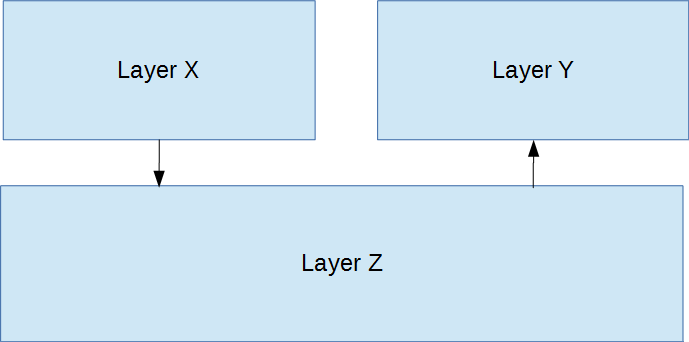
\includegraphics[width=0.60\textwidth]{images/layers}
 \caption{A simple architectural layer diagram}
\end{figure}

\subsection{Layer X Description}
Each layer should be described separately in detail. Descriptions should include the features, functions, critical interfaces and interactions of the layer. The description should clearly define the services that the layer provides. Also include any conventions that your team will use in describing the structure: naming conventions for layers, subsystems, modules, and data flows; interface specifications; how layers and subsystems are defined; etc. 

\subsection{Layer Y Description}
Each layer should be described separately in detail. Descriptions should include the features, functions, critical interfaces and interactions of the layer. The description should clearly define the services that the layer provides. Also include any conventions that your team will use in describing the structure: naming conventions for layers, subsystems, modules, and data flows; interface specifications; how layers and subsystems are defined; etc. 

\subsection{Layer Z Description}
Each layer should be described separately in detail. Descriptions should include the features, functions, critical interfaces and interactions of the layer. The description should clearly define the services that the layer provides. Also include any conventions that your team will use in describing the structure: naming conventions for layers, subsystems, modules, and data flows; interface specifications; how layers and subsystems are defined; etc. 
\section{Roles \& Responsibilities}
The immediate stakeholders of our project are the customers, sponsors, and developers. Customers are the ones who rely on the developers to create a product that meets their needs.They also rely on the sponsor to set expectations for the product. The sponsor funds the development of the idea, also sets expectations for the development of the product. Our point of contact for the sponsor will be Alex Escobar for app development, Hunter Walters for hardware development, and Haris Qureshi for embedded development.The point of contact for the customers will be Jeff Groenteman our sponsor. On the embedded development team we have Atafo Abure working with the app development team as well as Haris Qureshi and we have David Nguyen, Deion Nwaefulu, Aditya Rajguru working with the hardware development. The people working with the app development team will help set up communication from the app to the hub and the group working with the hardware team will help set up communication from the hub to each shutter. We split the team this way due to Atafo and Haris being CSE and David, Deion, and Aditya being CpE, this way we play to our strengths. We plan on maintaining the product owner and scrum master throughout the entirety of the project unless a change is mandatory. We choose to maintain the same scrum master due to consistency, meaning instead of having to change our method of scrum every so often, we can instead take our time getting used one scrum master.
\section{Cost Proposal}
We plan on making our product cost \$20, therefore we approximate our budget for \$40 to give ourselves some added leeway. The money will come from the \$800 budget we have from UTA. we expect the micro controller to be the most expensive item then the motor controller and motor. Currently these are our top expenses for the product. 

\subsection{Preliminary Budget}

\begin{table}[H]
\centering
\begin{tabular}{@{}|l|l|@{}}
\toprule
Item             & Cost (\$) \\ \midrule
Micro Controller & 6         \\ \midrule
Motor            & 2         \\ \midrule
Shutter          & 10        \\ \midrule
Gears            & 1         \\ \midrule
Wires            & 1         \\ \bottomrule
\end{tabular}
\caption{Preliminary Budget}
\label{tab:budget}
\end{table}



\subsection{Current \& Pending Support}
 Currently our only source of funding will be the \$800 from CSE department, we do not have any potential funding sources, we do not expect to go over budget. Our goal is to make an affordable and complete product that cost only \$20, we anticipate that our current budget should be more than enough.
\section{Facilities \& Equipment}
Currently we do not know everything we need, but what we do need is a labspace to develop the hardware portion of the shutters.We plan on using the Electrical Engineering Laboratory to construct the hardware. We will need shutters, a motor, a motor controller, a microcontroller, bluetooth adapters, iPhone, Android phone, and a computer to program everything. We are also planning on 3d printing our gears, which change the positioning the shutters, therefore we will need access to 3d printers. We realise if we 3D print out gears this will keep the cost of production low, but gears may need to be replaced more often as opposed to having gears made out of more durable materials such as aluminium, copper, chrome, nickel, steel, iron, or any other metal. We will also need a Wifi network to test the communication of the shutters on both bluetooth and Wifi. We also plan on developing apps for both Android and IOS therefore we will need two phones that run each operating system. We plan on developing the majority of the project in the Electrical Engineering lab simply due to the fact that the Electrical Engineering team will develop the hardware in this particular lab. We will not outsource any of our work, we are confident in our abilities, we also plan on purchasing bluetooth adapters, motor controllers, motors, and microcontrollers from online, currently we are unaware from which website but right now we are looking for affordable vendors. 

\section{Assumptions}
\begin{itemize}
  \item Only cost customers \$20, production should fall within \$15
  \item Installation time should be 10 minutes 
  \item The customer will provide network connectivity and ample power
  \item Shutters should follow an adjustable schedule
  \item Shutter should change  position on user request
  \item Each shutter should be unique and have an identifier
\end{itemize}
\section{Constraints}
\begin{itemize}
  \item Communication between three groups that is 16 people overall
  \item Research time for Bluetooth communication
  \item Lack of Knowledge on embedded development
  \item Keeping manufacturing cost less than \$15
  \item Making installation quick and simple
  \item Shutters remotely controlled by many users 
  \item Shutters have an adjustable schedule and be user adjusted 
  \item Shutters be battery powered
  \item Shutters should be ready for large scale production
\end{itemize}

\section{Risks}
\begin{table}[h]
\resizebox{\textwidth}{!}{
\begin{tabular}{|l|l|l|l|}
\hline
 \textbf{Risk description} & \textbf{Probability} & \textbf{Loss (days)} & \textbf{Exposure (days)} \\ \hline
 Availability of cheap motor & 0.10 & 2 & 0.20 \\ \hline
 Availability of compatible motor controller  & 0.20 & 3 & 0.60 \\ \hline
 Finding Affordable Micro Controller & 0.10 & 4 & 0.40 \\ \hline
 Delays in app development & 0.70 & 20 & 14 \\ \hline
 Delays in hardware development & 0.90 & 60 & 54 \\ \hline
 Delays in embedded development & 0.80 & 70 & 56 \\ \hline
\end{tabular}}
\caption{Overview of highest exposure project risks} 
\end{table}
\section{Documentation \& Reporting}
%%% In this section, you will describe all of the various artifacts that you will generate and maintain during the project life cycle. Describe the purpose of each item below, how the content will be generated, where it will be stored, how often it will be updated, etc. Replace the default text for each section with your own description. Reword this paragraph as appropriate.

\subsection{Major Documentation Deliverables}
\subsubsection{Project Charter}
This document will only be updated when or if there are any changes in our vision, mission, success criteria, system overview, roles, budget, equipment, facilities, constraints, or risks. We plan on delivering our initial version on Tuesday October 1, 2019. The final version will be delivered the last week of class.
\subsubsection{System Requirements Specification}
The system requirements document will be started once we figure out all of our system requirements and if anything changes we will update the document accordingly.  The initial version will be delivered on October 22, 2019 and the final version will be submitted the last week of class.

\subsubsection{Architectural Design Specification}
The Architectural design specification document initial version will be delivered November 12, 2019 and the final version will be submitted the last week of class. The document will be updated as needed, meaning if there are any changes in the architectural design this includes the finest details.

\subsubsection{Detailed Design Specification}
The Detailed Design specification document initial version will be delivered on December 2, 2019 and this will be the final version. We assume the document will not need any updating we plan on having all aspects of the project in order.

\subsection{Recurring Sprint Items}
\subsubsection{Product Backlog}
Items will be added to the product backlog as we work through the previous requirements and then get to the new requirements. All SRS items will go through thorough analysis before being added to the product backlog, to gain a full understanding of all customer needs .Item prioritization will be done by the team lead and will be prioritized by which items needs immediate attention. Product backlog will be shared and updated through Google Drive.

\subsubsection{Sprint Planning}
How will each sprint plan be planned? How many sprints will there be (you need to look at the schedules for this course and previous Senior Design II courses during the appropriate semesters to figure this out).

\subsubsection{Sprint Goal}
The team lead ultimately decides the sprint goal, but sprint goals are suggested by the entire team including the customer. Sprint goals will go through thorough analysis before being added. The customer will be either on call or in person when going over the sprint goals.

\subsubsection{Sprint Backlog}
Team lead will decide which product backlog items make their way into the sprint backlog, after informing the team and getting everyone's perspective on the task. The document will be maintained on Google Sheets. 

\subsubsection{Task Breakdown}
Tasks will be assigned by team members volunteering to claim a task. In order to document the time spent on a task will be through a time in time out portion on excel. Team members will enter the time they started a task and stop a task each day, then we will calculate the hours spent on the task. This will be in the scrum excel file.

\subsubsection{Sprint Burn Down Charts}
Team Lead is responsible for generating the burn down charts for each sprint. The charts will be on Google Sheets and shared with all team members, every member is expected to fill out the total amount of effort expended. Effort will be calculated by the number of tasks completed each day. The format of the sprint burn down chart will be x = days, y = task remaining, estimated effort line, and actual effort line.

\begin{figure}[h]
    \centering
    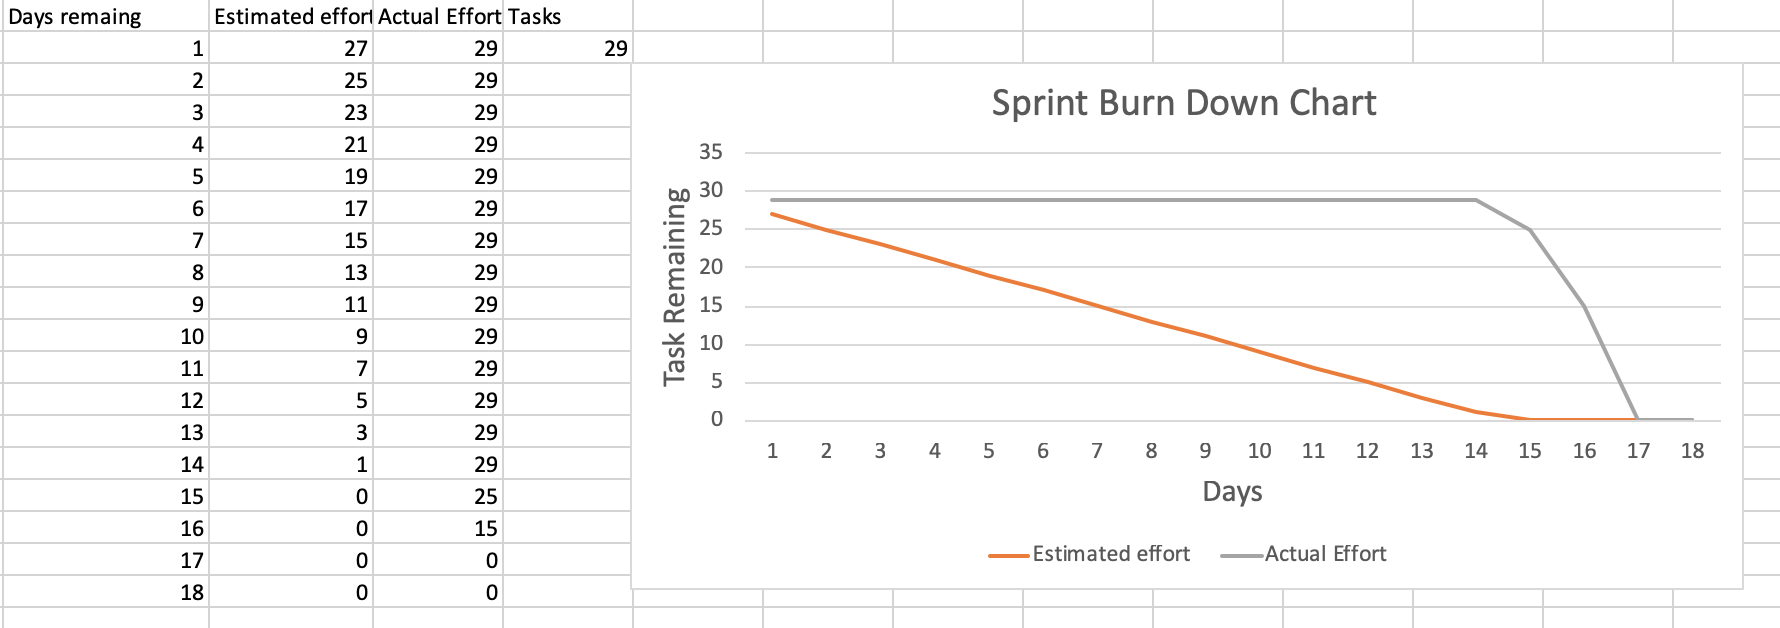
\includegraphics[width=0.5\textwidth]{images/SprintBurn}
    \caption{Example sprint burn down chart}
\end{figure}

\subsubsection{Sprint Retrospective}
There will be a sprint retrospective discussion the day after the sprint presentation. We will examine the sprint if there are any recurring items we will go over why it is recurring and if there is anything that we missed or could do better next sprint. Notes on what to improve on the next sprint will be documented as individuals. 


\subsubsection{Individual Status Reports}
Individual status reports will be after every sprint on the task each person completed. There will be a report of what they learned including resources they used it will also include what we need to focus on as a team. The key items will be a suggestion for next sprint and resources they used.

\subsubsection{Engineering Notebooks}
The engineering notebook will have no minimum number of pages completed for each interval, we are unaware of how long an interval will be. The notebook will be updated when there is a meeting with the sponsor or when meeting with other teams. The engineering notebook will be used mainly for notes when in meeting. There is no need to hold members accountable due to there being no minimum. The witness will be the team lead or higher, meaning product owner or the sponsor. This way team lead is constantly in the loop with all incoming ideas. 

\subsection{Closeout Materials}
\subsubsection{System Prototype}
The final system prototype will be demonstrated to the sponsor in person with a Prototype Acceptance Test (PAT) this way we are able to clearly show our progress to the sponsor and find any faults. We plan on presenting the prototype before the actual demo day two weeks before. The final system prototype will include the automatic shutter system and both the android and iOS apps. During the presentation we will show the shutter opening and closing with the app from user input and then from a schedule.

\subsubsection{Project Poster}
The poster will a 28x40 inches elmer's tri fold corrugated project display board, it will include pictures of the individual hardware components, pictures of both apps, a summary of what our product is capable of, who the intended customers are, and our goals for the future . The poster will be delivered on demo day. 

\subsubsection{Web Page}
We plan on making a simple informative website that will be available to the public and be delivered on demo day. It will include information about our product and will have the vision and mission portion of this document, it will include links to the apps and information on how to use the product and to set up the product. It will be provided at closeout.


\subsubsection{Demo Video}
The demo video will be over setting the product up, it will be a how to video uploaded to YouTube, we will include b-reel footage with a voice over and text going over how to install the product and setting up the Bluetooth communication through the app. The video will be approximately 20 minutes or less .

\subsubsection{Source Code}
We plan on having a Creative Common Software License this is to protect against hacking, also we can say what end users can and can not do. Source code will be maintained on a private GitHub repository, the customer will not be given the source code to prevent hacking the less people who know the code the better. The license terms will be in each source file and we still have to decide whether or not to make our project public.

\subsubsection{Source Code Documentation}
We plan on using Doxygen to generate documentation and the final documentation will be provided as a PDF available on the website.

\subsubsection{Hardware Schematics}
Will you be creating printed circuit boards (PCBs) or wiring components together? If so, list each applicable schematic and what sort of data it will contain (PCB layout, wiring diagram, etc.). If your project is purely software, omit this section.
Our portion of the project will be purely software

\subsubsection{Installation Scripts}
Customers will have to install the app on either IOS or Android and then follow the step by step process in setting up their smart shutter.

\subsubsection{User Manual}
The user manual will be available in the box with every product the manual will also be available on the website alongside a youtube video. The app will include step by step instructions on setting up the product. 

\newpage

%%% References
\bibliographystyle{plain}
\bibliographystyle{reference/IEEEtran_custom}
\bibliography{reference/refs}{}

\end{document}